\documentclass[border=8pt]{standalone}
\usepackage{fontspec}
\setmainfont{Source Serif 4}
\usepackage{pgfplots}
\pgfplotsset{compat=1.18}
\definecolor{qbase}{RGB}{31,86,160}
\colorlet{c1}{qbase!30}
\colorlet{c2}{qbase!50}
\colorlet{c3}{qbase!72}
\colorlet{c4}{qbase}
\definecolor{winner}{RGB}{209,73,91}

\begin{document}
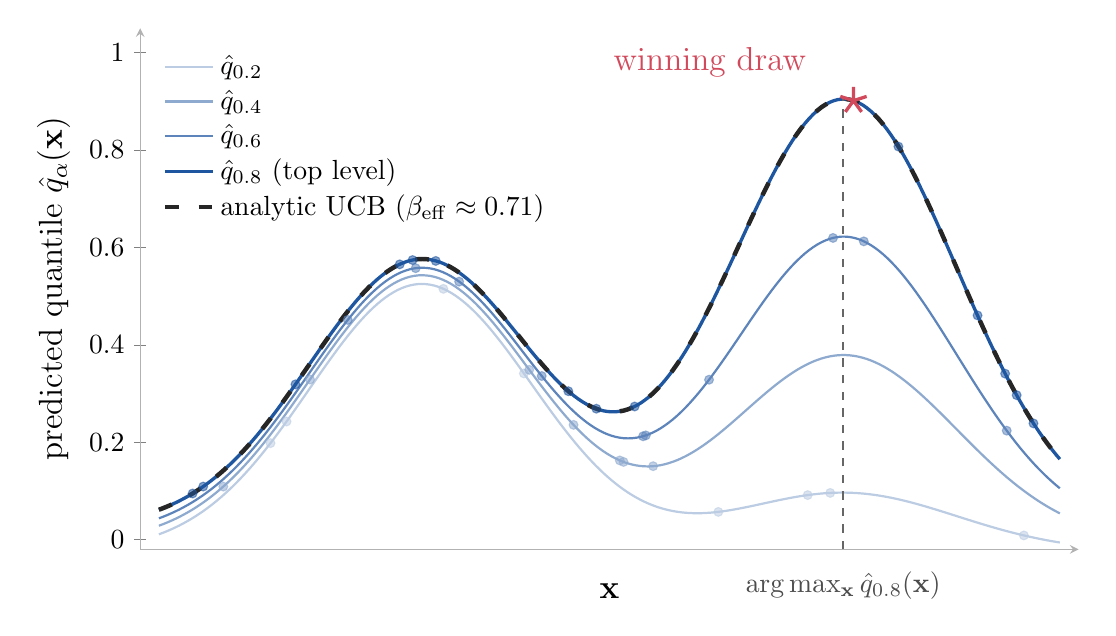
\begin{tikzpicture}[
  declare function={
    mmu(\x)=0.55*exp(-(\x-0.3)^2/(2*0.12^2)) + 0.5*exp(-(\x-0.75)^2/(2*0.12^2));
    ssg(\x)=0.03+0.45*exp(-(\x-0.75)^2/(2*0.12^2));
  }
]
\begin{axis}[
  width=13.5cm, height=8.2cm,
  axis lines=left,
  xlabel={$\mathbf{x}$}, ylabel={predicted quantile $\hat{q}_{\alpha}(\mathbf{x})$},
  xmin=0, xmax=1, ymin=-0.02, ymax=1.05,
  xticklabels={}, xtick style={draw=none},
  label style={font=\large},
  tick label style={font=\normalsize},
  legend style={at={(0.015,0.97)}, anchor=north west, font=\normalsize, draw=none,
                fill=white, fill opacity=0.85, text opacity=1},
  legend cell align=left,
  axis line style={gray!60},
  clip=false,
]
% quantile curves, light to dark with level
\addplot[domain=0.02:0.98, samples=220, thick, c1] {mmu(x) - 0.8416*ssg(x)};
\addlegendentry{$\hat{q}_{0.2}$}
\addplot[domain=0.02:0.98, samples=220, thick, c2] {mmu(x) - 0.2533*ssg(x)};
\addlegendentry{$\hat{q}_{0.4}$}
\addplot[domain=0.02:0.98, samples=220, thick, c3] {mmu(x) + 0.2533*ssg(x)};
\addlegendentry{$\hat{q}_{0.6}$}
\addplot[domain=0.02:0.98, samples=220, very thick, c4] {mmu(x) + 0.8416*ssg(x)};
\addlegendentry{$\hat{q}_{0.8}$ (top level)}
% analytic UCB at the grid-equivalent beta: coincides exactly (Gaussian predictive)
\addplot[domain=0.02:0.98, samples=220, line width=1.6pt, dash pattern=on 5pt off 7pt, black!85] {mmu(x) + 0.8416*ssg(x)};
\addlegendentry{analytic UCB ($\beta_{\mathrm{eff}} \approx 0.71$)}
% candidates, one dot per candidate at its drawn quantile (seed=1)
\addplot[only marks, mark=*, mark size=1.6pt, c1, opacity=0.55] coordinates { (0.3231,0.5149) (0.1560,0.2425) (0.4089,0.3412) (0.7353,0.0959) (0.7113,0.0914) (0.9417,0.0086) (0.1389,0.1981) (0.6161,0.0569) };
\addplot[only marks, mark=*, mark size=1.6pt, c2, opacity=0.55] coordinates { (0.5111,0.1626) (0.4146,0.3486) (0.5466,0.1508) (0.1810,0.3288) (0.5151,0.1595) (0.4618,0.2356) (0.0886,0.1089) };
\addplot[only marks, mark=*, mark size=1.6pt, c3, opacity=0.55] coordinates { (0.9234,0.2237) (0.4279,0.3359) (0.7383,0.6194) (0.5359,0.2122) (0.3399,0.5297) (0.7711,0.6124) (0.2212,0.4511) (0.2936,0.5573) (0.5388,0.2140) (0.6062,0.3283) };
\addplot[only marks, mark=*, mark size=1.6pt, c4, opacity=0.55] coordinates { (0.1655,0.3188) (0.9217,0.3408) (0.8080,0.8070) (0.0559,0.0947) (0.3150,0.5722) (0.4563,0.3047) (0.2766,0.5652) (0.4861,0.2688) (0.9519,0.2386) (0.9340,0.2966) (0.2903,0.5740) (0.8923,0.4604) (0.0672,0.1090) (0.5269,0.2733) };
% the winning draw
\addplot[only marks, mark=star, mark size=5pt, line width=1.2pt, winner] coordinates { (0.7601,0.9012) };
% argmax of the top-level curve
\draw[dashed, thick, black!60] (axis cs:0.7490,-0.02) -- (axis cs:0.7490,0.9044);
\node[anchor=north, font=\normalsize, black!70] at (axis cs:0.7490,-0.045)
  {$\arg\max_{\mathbf{x}} \hat{q}_{0.8}(\mathbf{x})$};
\node[winner, font=\large, anchor=south east] at (axis cs:0.72,0.93) {winning draw};
\end{axis}
\end{tikzpicture}
\end{document}
